% ============================================================
%  midsub_v2.tex -- EVS Project #19 Mid-Evaluation (version 2)
%  Structure: problem & motivation -> hypotheses -> methodology
%             -> preliminary analysis (H1, H2) -> things left to do
%
%  Compile (from slides/):  pdflatex midsub_v2; bibtex midsub_v2;
%                           pdflatex midsub_v2; pdflatex midsub_v2
%  Numbers: same sources as midsub.tex (see NUMBERS.md).
%  New figure: python slides/make_v2_figures.py
% ============================================================
\documentclass[11pt,aspectratio=169]{beamer}

\usetheme{Madrid}
\usecolortheme{seahorse}

\usepackage[T1]{fontenc}
\usepackage[utf8]{inputenc}
\usepackage{tikz}
\usetikzlibrary{positioning, arrows.meta, shapes.geometric}
\usepackage{booktabs}
\usepackage{graphicx}
\usepackage{multirow}
\usepackage{array}
\newcolumntype{L}[1]{>{\raggedright\arraybackslash}p{#1}}
\usepackage{natbib}
\bibliographystyle{unsrtnat}

\newcommand{\FigPath}[1]{../figures/#1.png}
\newcommand{\Fig}[2]{\includegraphics[width=#2,height=0.66\textheight,keepaspectratio]{\FigPath{#1}}}

\title[Compound Heat-Drought Stress]{Compound Heat--Drought Stress over India}
\subtitle{Are ecosystems hit harder when heat and drought strike together?\\[2pt]
  \small Mid-Evaluation, EVS Project \#19}
\author[Deshmukh et al.]{
  Arnav Deshmukh \and Ayush Brajesh Roy \and Saksham Chitkara \and
  Gracy Garg \and Rudra Choudhary
}
\institute{IIIT Hyderabad}
\date{\today}

\begin{document}

\frame{\titlepage}

\begin{frame}{Outline}
  \tableofcontents
\end{frame}

% =================================================================
\section{Problem statement \& motivation}
% =================================================================

\begin{frame}{Heat and drought rarely come alone}
  \small
  \begin{columns}[T]
    \column{0.48\linewidth}
    \begin{itemize}
      \item A \textbf{drought} is a shortage of water: little rain, dry soil.
      \item A \textbf{heatwave} is unusually high temperature, which makes the
        air ``thirstier'' (higher vapour-pressure deficit, VPD).
      \item They tend to happen \emph{together}:
        \begin{itemize}
          \item dry soil cannot cool the land by evaporation, so it heats up;
          \item heat raises evaporation, so soil dries even faster.
        \end{itemize}
      \item This loop is why heat--drought episodes can feed on themselves.
    \end{itemize}
    \column{0.5\linewidth}
    \centering
    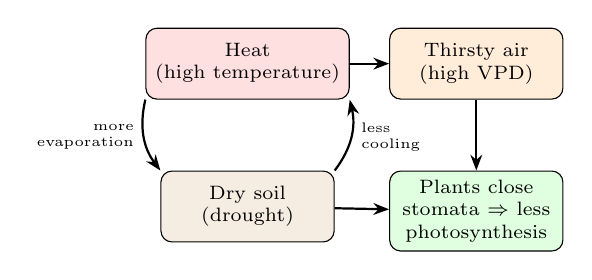
\begin{tikzpicture}[
        node distance=9mm and 5mm,
        b/.style={draw, rounded corners, align=center, font=\scriptsize,
                  minimum width=2.2cm, minimum height=0.9cm},
        a/.style={-{Stealth[length=2mm]}, thick}]
      \node[b, fill=red!12] (heat) {Heat\\(high temperature)};
      \node[b, fill=orange!15, right=of heat] (vpd) {Thirsty air\\(high VPD)};
      \node[b, fill=brown!15, below=of heat] (soil) {Dry soil\\(drought)};
      \node[b, fill=green!12, below=of vpd] (gpp) {Plants close\\stomata $\Rightarrow$ less\\photosynthesis};
      \draw[a] (heat) -- (vpd);
      \draw[a] (vpd) -- (gpp);
      \draw[a] (soil) -- (gpp);
      \draw[a] (heat.south west) to[bend right=25] node[left, font=\tiny, align=right]{more\\evaporation} (soil.north west);
      \draw[a] (soil.north east) to[bend right=25] node[right, font=\tiny, align=left]{less\\cooling} (heat.south east);
    \end{tikzpicture}
  \end{columns}
\end{frame}

\begin{frame}{Why it matters for ecosystems}
  \small
  \begin{itemize}
    \item Plants take up carbon through photosynthesis. This is \textbf{gross
      primary productivity (GPP)}: the base of food production and the land
      carbon sink.
    \item Under heat \emph{and} drought, plants are squeezed from both sides:
      \begin{itemize}
        \item less water available in the soil (drought);
        \item more water demanded by the air (heat), so plants close their
          stomata to avoid drying out and stop taking in CO$_2$.
      \end{itemize}
    \item Past events show the stakes:
      \begin{itemize}
        \item The 2003 European heat + drought cut productivity by about
          30\% and turned Europe's land into a temporary carbon
          \emph{source} \citep{ciais2005}.
        \item Across flux-tower sites worldwide, combined heat + drought reduced the
          carbon sink more than either extreme alone \citep{vonbuttlar2018}.
      \end{itemize}
    \item As the climate warms, more droughts will happen during hot
      spells. In India, concurrent droughts and heatwaves have become more
      frequent and widespread \citep{sharma2017}.
  \end{itemize}
\end{frame}

\begin{frame}{Why India?}
  \small
  \begin{columns}[T]
    \column{0.55\linewidth}
    \begin{itemize}
      \item \textbf{Monsoon dependence.} Most rain falls in June--September.
        A weak monsoon means drought (in our 1991--2024 data, 2002 was the
        driest year and 2009 the 5th driest).
      \item \textbf{Hot pre-monsoon.} March--May is already the hottest
        season. 2010 and 2022 were the 1st and 3rd hottest pre-monsoons
        in our data.
      \item \textbf{Land use.} Cropland is the dominant cover in about 60\%
        of India's grid cells, so lost productivity means lost food and
        income.
      \item \textbf{Research gap.} Most compound-event studies focus on
        Europe, China or the whole globe. India-wide work on vegetation is
        only just appearing \citep{meena2026,sen2026,malik2025}.
    \end{itemize}
    \column{0.43\linewidth}
    \centering
    \Fig{study_area_landcover}{\linewidth}\\[-2pt]
    {\tiny Dominant land cover (ESA WorldCover); red = cropland}
  \end{columns}
\end{frame}

\begin{frame}{Problem statement}
  \small
  \textbf{Assigned topic \#19:} \emph{Compound Heat--Drought Stress: are
  ecosystems experiencing stronger combined impacts?} Does simultaneous heat
  and drought produce greater ecosystem stress than either disturbance alone?
  Compare productivity and recovery during compound and single-stressor events.

  \vspace{6pt}
  \textbf{Our questions, for India:}
  \begin{enumerate}
    \item Is vegetation hit harder in compound (hot \emph{and} dry) months
      than in hot-only or dry-only months?
    \item Is the compound hit \emph{bigger than the heat damage plus the
      drought damage added together}?
      \begin{itemize}
        \item If \textbf{additive}: we can predict compound impacts from
          what we know about each stress separately.
        \item If \textbf{synergistic}: compound events are a distinct,
          more dangerous risk that single-stress studies would underestimate.
      \end{itemize}
    \item Do ecosystems take longer to recover after compound events?
    \item Does the answer differ between forests, croplands, grasslands,
      and between Peninsular and North India?
  \end{enumerate}
\end{frame}

\begin{frame}{What is known, and what is still open}
  \scriptsize
  \begin{columns}[T]
    \column{0.5\linewidth}
    \textbf{Known}
    \begin{itemize}
      \item Compound heat + drought hurts the carbon sink more than single
        extremes (flux towers: \citealp{vonbuttlar2018}; Europe 2003:
        \citealp{ciais2005}).
      \item India-wide, compound dry--hot conditions raise the
        \emph{probability} of vegetation drought, with amplification
        metrics on NDVI \citep{meena2026}.
      \item In Peninsular forests, compound hot--dry extremes raise the risk
        of large GPP losses \citep{sen2026}.
    \end{itemize}
    \column{0.5\linewidth}
    \textbf{Open}
    \begin{itemize}
      \item Is the effect on \emph{average} productivity super-additive, or
        just additive? Few studies test this directly, with uncertainty.
      \item Results depend on how drought is defined. Soil-based and
        atmosphere-based definitions give different impacts
        \citep{liang2026}.
      \item Recovery: global studies disagree on whether compound events
        delay recovery \citep{yao2024,huang2025} or not \citep{feng2026}.
        There is no India-specific comparison that we found.
    \end{itemize}
  \end{columns}
  \vspace{6pt}
  \textit{Our aim: an India-wide, honest test of additivity on two
  satellite measures, with uncertainty and a drought-index check, then
  recovery and regional differences. This is a regional synthesis with
  extensions, not a first-of-its-kind study.}
\end{frame}

% =================================================================
\section{Our hypotheses}
% =================================================================

\begin{frame}{Our hypotheses}
  \small
  \renewcommand{\arraystretch}{1.25}
  \begin{tabular}{@{}L{0.07\linewidth}L{0.52\linewidth}L{0.36\linewidth}@{}}
    \toprule
    & \textbf{Hypothesis} & \textbf{Status at mid-eval} \\
    \midrule
    \textbf{H1} & Vegetation (GPP, NDVI) is lower in compound months than in
      hot-only or dry-only months. & \textbf{Tested} (preliminary results) \\
    \textbf{H2} & The compound effect is \emph{synergistic}: larger than the
      heat effect + the drought effect. & \textbf{Tested} (preliminary results) \\
    \textbf{H3} & Ecosystems recover more slowly after compound events than
      after droughts. & Method built; for the final evaluation \\
    \textbf{H4} & The response differs by land cover and by region
      (Peninsular vs North India). & Method built; for the final evaluation \\
    \bottomrule
  \end{tabular}

  \vspace{6pt}
  \footnotesize Throughout, we check that conclusions do not depend on the
  choice of drought index (SPEI-3 vs SPI-3).
\end{frame}

% =================================================================
\section{Methodology}
% =================================================================

\begin{frame}{Data}
  \scriptsize
  \renewcommand{\arraystretch}{0.95}
  \begin{tabular}{@{}L{0.21\linewidth}L{0.33\linewidth}L{0.12\linewidth}L{0.27\linewidth}@{}}
    \toprule
    \textbf{Dataset} & \textbf{What we use} & \textbf{Period} & \textbf{Role} \\
    \midrule
    ERA5-Land \citep{munozsabater2021} & daily max temperature; soil moisture 0--100 cm; VPD & 1991--2024 & defines ``hot''; mechanism \\
    SPEI v2.11 \citep{vicenteserrano2010} & SPEI-3 (rain minus evaporative demand) & 1991--2024 & defines ``dry'' \\
    CHIRPS v2 \citep{funk2015} & rainfall $\rightarrow$ SPI-3 & 1991--2024 & temperature-free drought check \\
    MODIS MOD17A2H \citep{running2015,running2004} & GPP (photosynthesis) & 2001--2022 & main response \\
    MODIS MOD13A3 \citep{didan2021} & NDVI (greenness), quality-masked & 2001--2022 & second response \\
    ESA WorldCover \citep{zanaga2022} & land-cover fractions & 2021 & vegetation mask; land-cover groups \\
    \bottomrule
  \end{tabular}

  \vspace{6pt}
  \begin{itemize}
    \item All five suggested datasets, processed in Google Earth Engine
      \citep{gorelick2017} onto one common grid: 0.25\textdegree{} ($\approx$27 km),
      monthly, all of India (4,481 grid cells).
    \item GPP and NDVI both come from the MODIS Terra satellite: two
      different products, but not independent sensors.
  \end{itemize}
\end{frame}

\begin{frame}{Metrics at a glance}
  \scriptsize
  \renewcommand{\arraystretch}{1.0}
  \begin{tabular}{@{}L{0.14\linewidth}L{0.53\linewidth}L{0.27\linewidth}@{}}
    \toprule
    \textbf{Metric} & \textbf{What it measures} & \textbf{How to read it} \\
    \midrule
    \multicolumn{3}{@{}l}{\textit{Ecosystem response}} \\
    GPP & Carbon taken up by plants through photosynthesis (gC/m$^2$/month) & higher = more productive \\
    NDVI & Canopy greenness from red and near-infrared reflectance (0--1) & higher = greener \\
    \midrule
    \multicolumn{3}{@{}l}{\textit{Stress}} \\
    Tmax $z$ & Anomaly of the monthly mean daily maximum temperature & $\ge 1$: ``hot'' month \\
    SPEI-3 & 3-month water balance: rain minus evaporative demand & $\le -1$: ``dry'' month \\
    SPI-3 & 3-month rainfall only (no temperature in it) & $\le -1$: dry (robustness) \\
    Soil moisture & Water in the top 1 m of soil & lower = drier soil \\
    VPD & Vapour-pressure deficit: how ``thirsty'' the air is & higher = more water stress \\
    \midrule
    \multicolumn{3}{@{}l}{\textit{Statistics}} \\
    $z$-score & Distance from normal for that place and calendar month (in SDs) & 0 = normal; $-1$ = clearly low \\
    Amplification & Compound effect $-$ (heat effect + drought effect) & $<0$ synergy; $\approx0$ additive \\
    95\% CI & Year-block bootstrap: 1,000 resamples of whole years & excludes 0 = significant \\
    \bottomrule
  \end{tabular}
\end{frame}

\begin{frame}{Workflow}
  \centering
  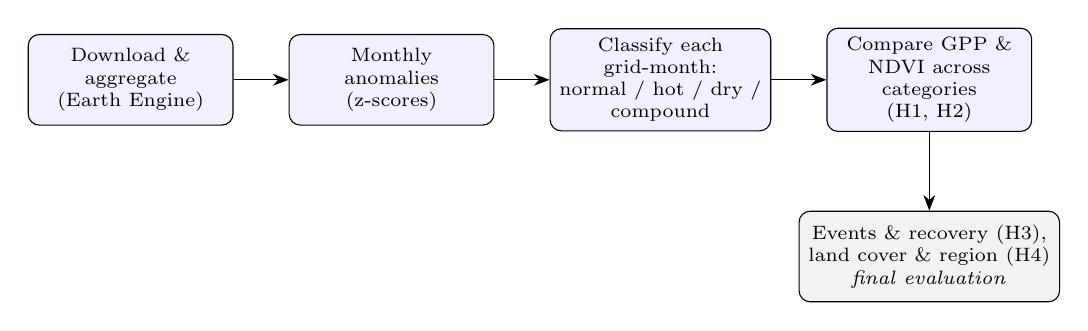
\begin{tikzpicture}[
      node distance=7mm,
      box/.style={draw, rounded corners, align=center, minimum width=2.6cm,
                  minimum height=1.15cm, font=\scriptsize, fill=blue!6},
      arr/.style={-{Stealth[length=2mm]}}]
    \node[box] (a) {Download \&\\aggregate\\(Earth Engine)};
    \node[box, right=of a] (b) {Monthly\\anomalies\\(z-scores)};
    \node[box, right=of b] (c) {Classify each\\grid-month:\\normal / hot / dry /\\compound};
    \node[box, right=of c] (d) {Compare GPP \&\\NDVI across\\categories\\(H1, H2)};
    \node[box, below=10mm of d, fill=gray!10] (e) {Events \& recovery (H3),\\land cover \& region (H4)\\\textit{final evaluation}};
    \draw[arr] (a) -- (b); \draw[arr] (b) -- (c); \draw[arr] (c) -- (d); \draw[arr] (d) -- (e);
  \end{tikzpicture}

  \vspace{10pt}
  \footnotesize Everything is scripted in Python (xarray, scipy, statsmodels)
  and checked by 68 automated tests. The analysis reruns from cached data in
  minutes.
\end{frame}

\begin{frame}{Step 1: anomalies (comparing like with like)}
  \small
  \begin{itemize}
    \item Raw values are not comparable: May is always hotter than January,
      and a desert always has less GPP than a forest.
    \item So for every grid cell and every calendar month, we convert a value
      into a \textbf{z-score}:
      \[
        z = \frac{\text{this month's value} - \text{normal for this cell in this month}}
                 {\text{typical year-to-year spread}}
      \]
      $z = -1$ means ``one standard deviation below what is normal here at
      this time of year''.
    \item \textbf{Temperature}: normal = 1991--2020. Not detrended, so
      long-term warming counts as heat.
    \item \textbf{GPP, NDVI}: a linear trend is removed first, so the
      long-term greening of India (CO$_2$, irrigation) is not mistaken for
      an anomaly.
    \item \textbf{Only growing-season months count}: the cell is in India,
      at least 50\% vegetated, and GPP in that month is normally at least
      30\% of its peak. This removes deserts and dormant seasons
      (824,598 grid-months remain).
  \end{itemize}
\end{frame}

\begin{frame}{Step 2: sorting every grid-month into four boxes}
  \begin{columns}
    \column{0.44\linewidth}
    \centering
    \renewcommand{\arraystretch}{1.4}
    \begin{tabular}{cc|c|c}
      & & \multicolumn{2}{c}{SPEI-3 (dryness)} \\
      & & $> -1$ & $\le -1$ \\
      \hline
      \multirow{2}{*}{Tmax $z$} & $< 1$ & Normal & Dry-only \\
      & $\ge 1$ & Hot-only & \textbf{Compound} \\
    \end{tabular}

    \vspace{6pt}
    \scriptsize
    \begin{tabular}{@{}lr@{}}
      Normal & 573,543 \\
      Hot-only & 79,717 \\
      Dry-only & 109,073 \\
      \textbf{Compound} & \textbf{62,265} (7.6\%) \\
    \end{tabular}
    \column{0.54\linewidth}
    \scriptsize
    \begin{itemize}
      \item \textbf{Hot}: the month's average daily maximum temperature is at
        least 1 standard deviation above normal.
      \item \textbf{Dry}: SPEI-3 $\le -1$, i.e.\ the last 3 months had
        clearly less water than usual (rain minus evaporative demand).
      \item SPEI's demand term depends on temperature, so ``dry'' is partly
        driven by heat. We therefore repeat everything with
        \textbf{SPI-3}, which uses rainfall only.
      \item Left: number of growing-season grid-months in each box, India,
        2001--2022.
    \end{itemize}
  \end{columns}
\end{frame}

\begin{frame}{Step 3: how we test H1 and H2}
  \small
  \begin{itemize}
    \item \textbf{H1}: average GPP $z$ (and NDVI $z$) in each box, and the
      differences between boxes.
    \item \textbf{H2}: compare the compound effect with the sum of the single
      effects. Each effect is measured relative to normal months:
      \[
        \text{Amplification} = \Delta_{\text{compound}} -
          \left(\Delta_{\text{hot}} + \Delta_{\text{dry}}\right)
      \]
      \vspace{-10pt}
      \begin{itemize}
        \item $< 0$: compound is worse than the sum $\Rightarrow$ \textbf{synergy};
        \item $\approx 0$: \textbf{additive};
        \item $> 0$: less than the sum (\textbf{sub-additive}).
      \end{itemize}
    \item \textbf{Uncertainty}: 95\% confidence intervals from a
      \emph{year-block bootstrap}. We resample whole years (1,000 times), because
      neighbouring cells in the same year are not independent. A result is
      called significant when its interval excludes zero.
  \end{itemize}
\end{frame}

% =================================================================
\section{Preliminary analysis (H1, H2)}
% =================================================================

\begin{frame}{Data check: do the inputs reproduce known events?}
  \centering
  \Fig{qc_jjas_anomalies}{0.7\linewidth}

  \scriptsize India-mean SPEI-3 at the end of the monsoon: 2002 is the driest
  of 34 years and 2009 the 5th. Pre-monsoon (Mar--May) Tmax: 2010 is the hottest
  of 34 years and 2022 the 3rd. The inputs pick up the real droughts and
  heatwaves.
\end{frame}

\begin{frame}{Where compound months happen}
  \begin{columns}
    \column{0.5\linewidth}
    \centering
    \Fig{freq_map_compound}{\linewidth}
    \column{0.48\linewidth}
    \small
    \begin{itemize}
      \item Share of each cell's growing-season months that were compound,
        2001--2022.
      \item Overall, 7.6\% of growing-season grid-months are compound.
      \item Hotspots: the northern plains, east-central India, the
        North-East, and a belt in the western Deccan (around 15--18\textdegree N).
      \item Both North and Peninsular India have more than 20,000 compound
        grid-months, enough for a reliable comparison.
    \end{itemize}
  \end{columns}
\end{frame}

\begin{frame}{H1: is vegetation hit harder in compound months?}
  \centering
  \Fig{composite_gpp_z_overall}{0.47\linewidth}
  \hfill
  \Fig{composite_ndvi_z_overall}{0.47\linewidth}

  \scriptsize
  \begin{tabular}{@{}lcccc@{}}
    \toprule
    Mean $z$ [95\% CI] & Normal & Hot-only & Dry-only & Compound \\
    \midrule
    GPP  & $+0.12$ & $-0.13$ [$-0.24,-0.01$] & $-0.27$ [$-0.40,-0.15$] & $\mathbf{-0.43}$ [$-0.54,-0.33$] \\
    NDVI & $+0.19$ & $-0.37$ [$-0.50,-0.26$] & $-0.30$ [$-0.41,-0.21$] & $\mathbf{-0.68}$ [$-0.81,-0.55$] \\
    \bottomrule
  \end{tabular}
\end{frame}

\begin{frame}{H1: result}
  \small
  \begin{itemize}
    \item All three stress types lower productivity and greenness
      significantly compared with normal months.
    \item \textbf{Compound months are the worst}, and significantly worse
      than either single stress:
      \begin{itemize}
        \item compound minus dry-only: GPP $-0.16$ [$-0.26,-0.04$],
          NDVI $-0.38$ [$-0.49,-0.28$];
        \item compound minus hot-only: GPP $-0.30$ [$-0.40,-0.21$],
          NDVI $-0.31$ [$-0.43,-0.21$].
      \end{itemize}
    \item Robust to the drought index. With rainfall-only SPI-3, compound
      minus dry-only is GPP $-0.26$ [$-0.37,-0.13$] and NDVI $-0.48$
      [$-0.61,-0.35$].
    \item \textbf{Why?} Compound months combine the driest soils \emph{and}
      the thirstiest air:

      \vspace{2pt}
      \scriptsize
      \begin{tabular}{@{}lcccc@{}}
        \toprule
        & Normal & Hot-only & Dry-only & Compound \\
        \midrule
        Root-zone soil moisture $z$ & $+0.29$ & $-0.75$ & $-0.38$ & $\mathbf{-1.04}$ \\
        Air dryness (VPD) $z$ & $-0.38$ & $+1.11$ & $+0.18$ & $\mathbf{+1.43}$ \\
        \bottomrule
      \end{tabular}
  \end{itemize}
  \vspace{2pt}
  \textbf{H1 supported.}
\end{frame}

\begin{frame}{H2: is the combination worse than the sum?}
  \centering
  \includegraphics[width=0.92\linewidth]{\FigPath{additivity_gpp_ndvi}}

  \scriptsize Hatched bar: what we would expect if the two damages simply
  added up. Green bar: what actually happened in compound months.
\end{frame}

\begin{frame}{H2: result}
  \begin{columns}[T]
    \column{0.5\linewidth}
    \small
    Amplification $= \Delta_{\text{compound}} - (\Delta_{\text{hot}} +
    \Delta_{\text{dry}})$; $<0$ would mean synergy.

    \vspace{6pt}
    \begin{tabular}{@{}lrr@{}}
      \toprule
      & with SPEI-3 & with SPI-3 \\
      \midrule
      GPP  & $+0.09$ & $-0.00$ \\
           & \scriptsize[$-0.03$, $+0.21$] & \scriptsize[$-0.12$, $+0.13$] \\
      NDVI & $+0.18$ & $+0.06$ \\
           & \scriptsize[$+0.06$, $+0.30$] & \scriptsize[$-0.05$, $+0.18$] \\
      \bottomrule
    \end{tabular}
    \column{0.48\linewidth}
    \small
    \begin{itemize}
      \item \textbf{No synergy}: the amplification is never significantly
        negative.
      \item Heat and drought damages roughly \textbf{add up}. Compound
        months are worse than either alone, but not worse than both
        together.
      \item With SPEI-3, NDVI is even slightly \emph{less} than additive,
        but this disappears with SPI-3. The drought definition matters.
    \end{itemize}
  \end{columns}
  \vspace{6pt}
  \small \textbf{H2 not supported} (for average productivity, India-wide).
\end{frame}

\begin{frame}{H2: response surface (no boxes)}
  \begin{columns}
    \column{0.5\linewidth}
    \centering
    \Fig{response_surface_gpp}{\linewidth}
    \column{0.48\linewidth}
    \small
    \begin{itemize}
      \item Average GPP $z$ for every combination of temperature anomaly
        (x) and SPEI-3 (y), in steps of 0.5. Sparse bins ($<30$ values) are
        blank.
      \item GPP falls steadily as conditions get drier (from about $+0.5$ in
        the wettest rows to about $-0.35$ in the driest).
      \item The lowest bin is the hottest and driest corner ($-0.92$).
        Warm but wet months are \emph{above} normal.
      \item Consistent with roughly additive effects: dryness is the main
        driver, and heat adds to it.
    \end{itemize}
  \end{columns}
\end{frame}

\begin{frame}{Observations so far}
  \small
  \begin{itemize}
    \item \textbf{H1 supported.} Compound heat--drought months reduce
      productivity (GPP) and greenness (NDVI) significantly more than heat
      alone or drought alone. This holds for both drought indices.
    \item \textbf{H2 not supported.} The compound effect is about the
      \emph{sum} of the heat and drought effects, not more.
    \item \textbf{Mechanism.} Compound months have the driest soils and the
      thirstiest air at the same time.
    \item \textbf{Drought definition matters.} SPEI vs SPI changes the H2
      details. Hot-only months also have dry soils (soil moisture
      $z = -0.75$), which rainfall-based indices miss.
    \item \textbf{How this fits the literature.} \citet{meena2026} report
      ``nonlinear amplification'' for India using \emph{probabilities} of
      vegetation drought. Our test on \emph{average} anomalies finds
      additivity. The two ask different questions; comparing them directly
      is planned.
    \item \textbf{Caveats.} MOD17 GPP is partly modelled (it uses air
      dryness and temperature, and has no soil-moisture input). NDVI is from
      the same satellite. Monthly 0.25\textdegree{} data blur short
      heatwaves.
  \end{itemize}
\end{frame}

% =================================================================
\section{Things left to do}
% =================================================================

\begin{frame}{Improving H2: from four boxes to a regression}
  \footnotesize
  \textbf{Now:} each month goes into one of four boxes (normal / hot / dry
  / compound) using cut-offs at $\pm1$, and we compare box averages.

  \vspace{4pt}
  \textbf{Planned:} use the actual heat and dryness values for every month
  and fit
  \[
    \text{GPP}_z = a \times \text{heat} + b \times \text{dryness}
      + c \times (\text{heat} \times \text{dryness}) + \text{cell effect} + \varepsilon
  \]
  with heat = Tmax $z$ and dryness = $-$SPEI-3.
  \begin{itemize}
    \item $a$, $b$: how much GPP drops per unit of heat or dryness on its own.
    \item $c$: the \textbf{interaction}. $c < 0$ means heat hurts more when it
      is also dry, which is synergy, tested directly as one number with a CI.
    \item Better because:
      \begin{itemize}
        \item no arbitrary cut-offs;
        \item uses the full strength of each anomaly, not just in/out of a box;
        \item can add controls (season, land cover, earlier soil moisture);
        \item gives effect sizes per unit of stress.
      \end{itemize}
    \item Checks: compare with the response surface; repeat for NDVI and SPI-3;
      year-clustered uncertainty.
  \end{itemize}
\end{frame}

\begin{frame}{H3 and H4: planned analyses}
  \footnotesize
  \begin{columns}[T]
    \column{0.5\linewidth}
    \textbf{H3: recovery}
    \begin{itemize}
      \item Detect events: runs of $\ge2$ dry months (compound if any month
        is hot), and heat-only runs.
      \item Recovery time: months until GPP is back near normal
        ($z \ge -0.5$ for 2 months).
      \item Kaplan--Meier curves, so that unfinished recoveries are handled
        properly.
      \item Compare compound vs drought-only \emph{at the same drought
        severity}, since compound droughts tend to be longer and more
        severe.
      \item Test what drives recovery: rain after the event or air dryness
        (the studies disagree: \citealp{yao2024,huang2025,feng2026}).
    \end{itemize}
    \column{0.5\linewidth}
    \textbf{H4: land cover \& region}
    \begin{itemize}
      \item Repeat H1/H2 for forests, croplands, grasslands and shrublands.
      \item Peninsular (south of 22\textdegree N) vs North India, with a
        direct test of the difference.
      \item Split Peninsular forests into deciduous and evergreen.
      \item Map where (if anywhere) the effect is synergistic, cell by cell.
    \end{itemize}

    \vspace{4pt}
    \scriptsize The code for both is built and tested. Results will be
    finalised and presented at the final evaluation.
  \end{columns}
\end{frame}

\begin{frame}{Other planned work}
  \footnotesize
  \begin{itemize}
    \item \textbf{Independent productivity data.} Check GPP with a product
      built differently from MOD17 (e.g.\ PML or SIF-based GPP, as used by
      \citealp{sen2026}). MOD17 has built-in temperature and air-dryness
      responses, and satellite GPP is known to under-respond in forests
      \citep{flach2021}.
    \item \textbf{Stricter compound definition.} Require $\ge$50\% of a
      drought's months to be hot, and try daily heatwave definitions.
    \item \textbf{Sensitivity checks.}
      \begin{itemize}
        \item Thresholds of 1.28 SD instead of 1.
        \item 1- and 6-month SPEI.
        \item A soil-moisture-based drought definition (cf.\ \citealp{liang2026}).
        \item A one-month lag.
      \end{itemize}
    \item \textbf{Compare with \citet{meena2026}.} Compute a
      probability-based amplification metric alongside ours.
    \item \textbf{Case studies.} 2009 drought, 2015 drought, and the 2022
      pre-monsoon heatwave.
    \item \textbf{Final report}, with corrected references from our
      literature review.
  \end{itemize}
\end{frame}

\begin{frame}[allowframebreaks]{References}
  \footnotesize
  \bibliography{references}
\end{frame}

\end{document}
